%Tarea1

% --- Clase de archivo ---
% Con este comando se define que tipo de documento vamos a hacer
% en este caso un articulo, en una hoja a4 y con tamanio de fuente 11pt.
\documentclass[a4paper,12pt]{article}
% los tamanios mas utilizados son 10,11 y 12 pt y representan un tamanio de referencia, o sea que al cambiar a 12 pt todos los textos van a aumentar proporcionalmente, al estilo homotecia.


% A partir de aqui se definiran ciertos paquetes o funciones a ser utilizadas
% dentro del documento.


% --- codificacion de archivo ---
% El paquete inputenc sirve para que el compilador pueda interpretar los acentos en espaniol de forma estandar, dependiendo del sistema operativo hay que darle una configuracion diferente:
\usepackage[utf8]{inputenc}
% ----------------------------------


% --- idioma ---
% El paquete babel sirve para separar correctamente las palabras en muchos idiomas, aquií­ esta configurado con espaniol (spanish). Tambien sirve para que el Ií­ndic etenga tií­tulo "Indice" en lugar de "Contents".
\usepackage[spanish]{babel} 
% --------------


% --- Fuentes ---
% El paquete fontenc sirve para controlar las fuentes que utiliza el documento
\usepackage[T1]{fontenc}
% Si dejamos comentado el paquete de abajo utilizaremos la fuente por defecto
% si se quita el comentario se usa sans. Se puede usar times, y otras opciones que se dejan comentadas. 
%\usepackage{sans}
%\usepackage{fbb}
%\usepackage{bera}
%\usepackage{sans}
%\usepackage{times}
%\usepackage{libertine} 


\usepackage{dirtytalk} % Paquete para facilitar la notación de citas con el comando \say{}



% --- Gráficos ---
% El paquete graphicx sirve para controlar figuras con \includegraphics.
\usepackage{graphicx}
% Esta linea indica el lugar (path) en el cual se encuentra la carpeta donde colocamos imágenes, para ahorrar colocarlo en cada
% llamado de una imagen en el documento.
\graphicspath{{./figuras/}}
% Estos paquetes permiten colocar varias figuras en el entorno "figure" como subfiguras (cualquiera de los dos).
\usepackage{float}
\usepackage{subfig} 


% --- Lenguaje matemático ---
% fuentes para escribir sí­mbolos
\usepackage{amsfonts,amssymb,amsthm,amsmath}


% --- Tablas ---
% Paquetes para el manejo de tablas, creación de filas y columnas unidas.
\usepackage{multirow} 
\usepackage{multicol} 
% Control de color en tablas muy versátil.
\usepackage[table]{xcolor}


% --- Hipervínculos ---
% paquete para marcar los hiperví­nculos en i­ndice y referencias
\usepackage{hyperref}
% Para citar referencias  
\usepackage{cite} 
\hypersetup{colorlinks, urlcolor=cyan, citecolor=green, linkcolor=blue} % Pinta con color las referencias
\usepackage[hypcap]{caption} % Las imágenes tienen hiperreferencia y se ven completas y no solo la leyenda. 
% Para hacer hiperreferencias a páginas web
\usepackage{url} 


\usepackage{booktabs} 

% --- Numeración ---
% Paquete que cambia como se representa la numeración de las imágenes, ecuaciones y tablas
\usepackage{chngcntr}
% Ahora se nombran por sección reiniciando el conteo en cada sección
\counterwithin{figure}{section}
\counterwithin{equation}{section}
\counterwithin{table}{section}


% Para agregar al índice las refencias
\usepackage[nottoc,notlot,notlof]{tocbibind} 



% Aqui comienzan los datos del trabajo. El comando \date{\today} asigna la fecha en que se compila como la fecha del trabajo, tambien se puede escibe directamente, ej. \date{5 de setiembre de 2012}.

\title{Tarea 4 Problemas conceptuales} 
\author{%
  Iván David Valderrama Corredor\\ %
  Ingeniería de Sistemas y Ciencias de la Computación\\ %
  Pontificia Universidad Javeriana, Cali}
\date{\today}
% ------------------------

%\pagestyle{empty}
% ====================================


%El paquete colortbl sirve para darle color a las tablas
\usepackage{colortbl}

% Este paquete se utiliza para generar texto de relleno.
\usepackage{blindtext}

% este paquete determina que el texto tenga como fuente normal: times, consultar el eva de latex para mas opciones.
%\usepackage{times}


% ===== Encabezado =====
% esta es una posible configuración para el encabezado. 
%Si se comentan estas dos lineas no habrá encabezado y la numeración de página aparecerá abajo de cada hoja. En la página donde se llame a \maketitle no se coloca encabezado.
\pagestyle{myheadings}
\markright{}
% ======================


%% ===== Ajuste layout pagina =====
% define el ancho del texto en la hoja
\setlength{\textwidth}{155mm}
% define el alto del texto en la hoja
\setlength{\textheight}{210mm}
% los márgenes pueden ser editador con
\oddsidemargin=-.25cm
%% ================================

% --- commandos definidos a gusto del usuario ---
\newcommand{\ds}{\displaystyle}
\def\x{{\bf x}}

\newcommand{\subfigureautorefname}{\figureautorefname}

% -----------------

% =====================================================
% =====================================================
\usepackage{listings}



% =====================================================
% ========  Aca comienza el cuerpo del texto ==========
%
\begin{document}
	
% Se renuevan comandos ya existentes de LaTeX como se desee, en este caso del nombre de tablas y figuras.	
\renewcommand{\tablename}{\bfseries Tabla} % Cambia nombre de tablas
\renewcommand{\figurename}{\bfseries Figura} % Cambia nombre de figuras 
%\newcommand{\subfigureautorefname}{\figureautorefname} % Para que al referenciar una subfigura aparezca "Figura"	
% Se refiere a las tablas y figuras con el comando \autoref{label} para que aparezca referenciado automáticamente el nombre de lo referenciado (Tabla o Figura) continuado por el número de la misma.	
%
% El comando \verb+maketitle+ sirve para escribir la cabecera con los datos del trabajo (título, autor y fecha).
\maketitle

% índice
\tableofcontents

% para separar la carátula del texto introducimos un salto de pagina
\newpage

% definimos una sección con el comando section

\section{Problemas conceptuales}

\subsection{Ejercicio 3.5:Binary Trees(Kleinberg y Tardos, página 108).}
Un árbol binario es un árbol arraigado en el que cada nodo tiene como máximo dos hijos. Muestre por inducción que en cualquier árbol binario el número de nodos con dos hijos es exactamente uno menos que el número de hojas.\\\\
\textbf{Respuesta}\\\\
Caso Base:\\\\
Consideremos el primer nodo(raiz), el cual puede tener de 0 a 2 hojas.\\\\
-Si la raíz no tiene hijos entonces la raiz es una hoja y el árbol solo tiene 1 hoja, por lo que no tiene nodos con 2 hijos.\\
-Si la raíz tiene unicamente una hoja, entonces el arbol solo tiene 1 hoja y no tiene nodos con 2 hijos.\\
-Si la raíz tiene dos hojas, entonces el árbol tiene 2 hojas y cada nodo tiene 2 hijos.\\\\
Hipótesis inductiva:\\\\
$P(n):$ En un arbol binario con n nodos, el numero de nodos con dos hijos es exactamente $(n-1)$.
\\\\
Supongamos que $P(n)$ es verdadero.\\\\
Caso1:\\
Tenemos un arbol binario con n+1 nodos, ahora agregaremos una hoja a un padre con solo un hijo.\\
Para este caso, el numero de nodos con dos hijos y hojas aumenta en 1\\\\
Caso2:\\
Tenemos un arbol binario con n+1 nodos, ahora agregaremos una hoja a un padre que es una hoja.\\
Para este caso, los padres con dos hijos y el numero de hojas siguen siendo iguales.
\cite{CourseH}\\\\
\subsection{Ejercicio 3.7:Wireless Networks(Kleinberg y Tardos, página 108).}
Algunos de tus amigos trabajan en redes inalámbricas y actualmente están estudiando las propiedades de una red de dispositivos móviles. A medida que los dispositivos se mueven (en realidad, cuando sus dueños humanos se mueven), definen un gráfico en cualquier momento como sigue: hay un nodo que representa cada uno de los n dispositivos, y hay un borde entre el dispositivo i y el dispositivo j si el dispositivo físico Las ubicaciones de i y j no están a más de 500 metros de distancia. (si es así, digamos que i y j) están "dentro del rango" el uno del otro.)\\
Les gustaría que la red de dispositivos esté conectada en todo momento, por lo que han restringido el movimiento de los dispositivos para satisfacer los siguientes requisitos: en todo momento, cada dispositivo está a 500 metros de al menos n / 2 de los otros dispositivos. (Asumiremos que n es un número par). Lo que les gustaría saber es: ¿Esta propiedad por sí misma garantiza que la red permanecerá conectada?\\\
Decida si cree que la afirmación es verdadera o falsa, y proporcione una prueba de la reclamación o su negación.\\\\
\textbf{Respuesta}\\\\
Supongamos que tenemos un grafo G(n,v)\\
En la primera capa del grafo tenemos $(n/2)+1$ canditad de vertices, en la segunda capa del grafo tenemos $(n/2)-1$ cantidad de vertices y asi sucesivamente hasta n. Cuando la cantidad de nodos es negativa, se empieza a reutilizar los nodos previamente empleados, enlazando caminos con dichos nodos, lo que prueba que el la red permanecera conectada, pues este grafo es un grafo conexo.\\\\
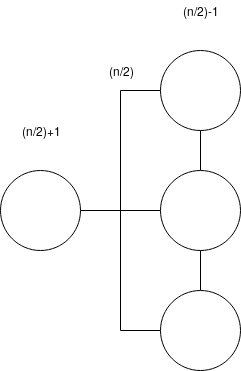
\includegraphics[scale=0.5]{punto2.png}\\
\subsection{Ejercicio 4.2:Minimum Spanning Trees(Kleinberg y Tardos, página 189).}
Para cada una de las siguientes dos afirmaciones, decida si es verdadero o falso. Si es verdad, da una breve explicación. Si es falso, da un contraejemplo.\\\\
(a) Suponga que se nos da una instancia del Problema del árbol de expansión mínima en un grafo G, con costos de borde que son todos positivos y distintos. Sea T un árbol de expansión mínimo para esta instancia. Ahora supongamos que reemplazamos cada costo de borde por su cuadrado, $c^{2}_{e}$. creando así una nueva instancia del problema con el mismo grafo pero con diferentes costos. ¿Verdadero o falso? T debe ser un árbol de expansión mínimo para esta nueva instancia.\\\\
\textbf{Respuesta}\\
Dado un arreglo de costos de arcos ordenados de manera creciente.\\
$A = [c_1,c_2,c_3...c_{n-1}]$\\
se cumple la siguiente propiedad\\
si $c_1 < c_2$ entonces $(c_1)^2 < (c_2)^2$\\
y esto se cumple para cualquier $c_n$\\
Ahora debido a que el orden del arreglo no es afectado al momento de reemplazar los costos por el cuadrado de los mismos, el arbol de expansion minima no cambia, por lo que el enunciado es verdadero.\\\\
(b) Supongamos que se nos da una instancia del problema de ruta s-t más corta en un grafo dirigido G. Suponemos que todos los costos de borde son positivos y distintos. Sea P una ruta s-t de costo mínimo para esta instancia. Ahora supongamos que reemplazamos cada costo de borde por su cuadrado, $c^{2}_{e}$, creando así una nueva instancia del problema con el mismo grafo pero con diferentes costos. ¿Verdadero o falso? P debe seguir siendo una ruta s-t de costo mínimo para esta nueva instancia.\\\\
\textbf{Respuesta}\\
Si tenemos el siguiente grafo:\\
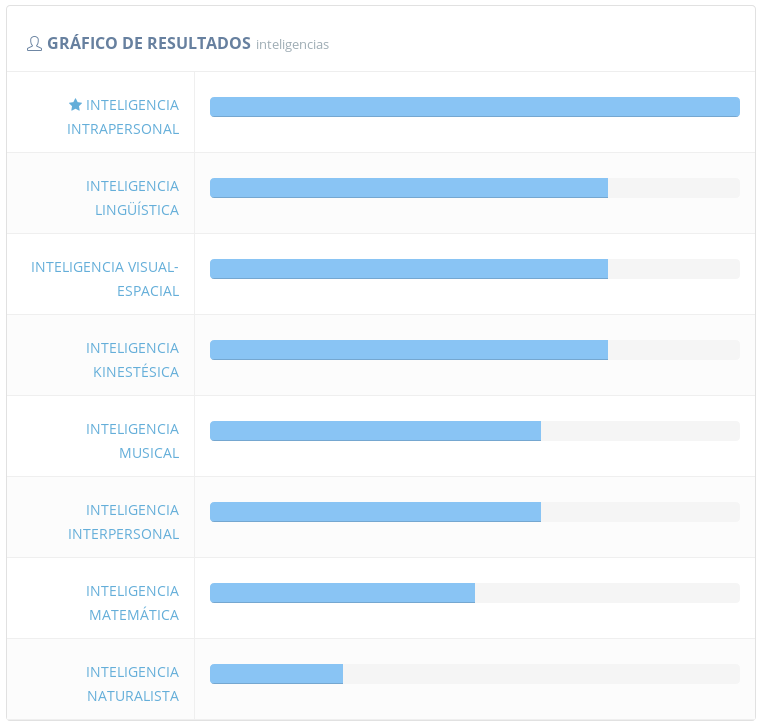
\includegraphics[scale=0.65]{img1.png}\\
La nueva instacia seria la siguiente:\\
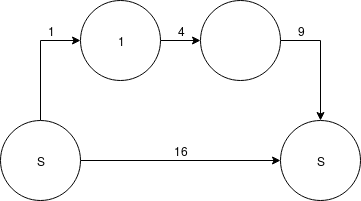
\includegraphics[scale=0.65]{img2.png}\\
Como podemos ver en la primera instancia del grafo, el camino empleado es el de (S,F)4=4. < (S,1,2,F)1+2+3=6\\
En cambio en la segunda instancia del grafo, el camino empleado es el\\
(S,1,2,F)1+4+9=14 < (S,F)16=16.\\\\
\subsection{Ejercicio 4.5:Quiet Country Roads(Kleinberg y Tardos, página 191).}
Consideremos un camino rural largo y tranquilo con casas dispersas muy dispersas a lo largo. (Podemos imaginar la carretera como un segmento de línea larga, con un punto final oriental y un punto final occidental).\\
Además, supongamos que a pesar de la configuración bucólica, los residentes de todas estas casas son ávidos usuarios de teléfonos celulares. Desea colocar estaciones base de teléfonos celulares en ciertos puntos a lo largo de la carretera, de modo que cada casa esté a cuatro millas de una de las estaciones base.\\
Proporcione un algoritmo eficiente que logre este objetivo, utilizando la menor cantidad de estaciones base posibles\\\\
\textbf{Respuesta}\\\\
Entrada: Un arreglo P[0..N] de numeros naturales, los cuales representan las posiciones de las casas\\
Salida: Numero Natural A que representa la cantidad minima de estaciones base empleadas, tal que cubran 4 millas de distancia por casa.
\lstinputlisting{Punto1.py}
\cite{CR}\\\\
\clearpage
% =====================
\begin{thebibliography}{15}

\bibitem{CourseH}
  Course Hero,
  \emph{Problem 9 a binary tree is a rooted tree in which}.\\
  https://www.coursehero.com/file/p5sovqg/Problem-9-A-binary-tree-is-a-rooted-tree-in-which-each-node-has-at-most-two/

\bibitem{CR}
  Camilo Rocha ,
  \emph{Minimal Covering Algorithm with failure checking}.\\
  https://https://bitbucket.org/snippets/hquilo/z6KbA
  
\end{thebibliography}

% =====================

\end{document}
